% =====================================================================
%  ViperGPT Reproduction — C1–C4 Prompt Specification Study
%  Professor-facing explanation notes
%
%  Compile:  pdflatex viper_c1c4_notes
%            pdflatex viper_c1c4_notes      (twice, for the ToC)
%
%  Self-contained: no bibliography, no external figures required.
% =====================================================================
\documentclass[11pt,a4paper]{article}

\usepackage[a4paper,margin=2.4cm]{geometry}
\usepackage[T1]{fontenc}
\usepackage[utf8]{inputenc}
\IfFileExists{lmodern.sty}{\usepackage{lmodern}}{}
\usepackage{amsmath,amssymb}
\usepackage{booktabs}
\usepackage{array}
\usepackage{xcolor}
\usepackage{listings}
\usepackage{enumitem}
\usepackage{caption}
\usepackage{tikz}
\usepackage{mdframed}
\usepackage[hidelinks]{hyperref}
\usetikzlibrary{shapes.geometric, arrows.meta, positioning, fit, backgrounds, calc}

% ---------------------------------------------------------------- palette
\definecolor{navy}{RGB}{18,42,86}
\definecolor{gold}{RGB}{184,138,40}
\definecolor{teal}{RGB}{31,111,120}
\definecolor{midgrey}{RGB}{120,126,134}
\definecolor{softgrey}{RGB}{242,243,245}
\definecolor{good}{RGB}{22,110,72}
\definecolor{bad}{RGB}{158,42,42}
\definecolor{codebg}{RGB}{248,248,250}

\newcommand{\up}[1]{\textcolor{good}{\textbf{#1}}}
\newcommand{\down}[1]{\textcolor{bad}{\textbf{#1}}}

% ---------------------------------------------------------------- code
\lstdefinestyle{py}{
  language=Python, basicstyle=\ttfamily\small,
  keywordstyle=\color{navy}\bfseries, stringstyle=\color{good},
  commentstyle=\color{midgrey}\itshape, backgroundcolor=\color{codebg},
  frame=leftline, framerule=1.4pt, rulecolor=\color{gold},
  xleftmargin=10pt, framexleftmargin=8pt, breaklines=true,
  showstringspaces=false, aboveskip=8pt, belowskip=8pt,
}
\lstdefinestyle{plainlist}{
  language={}, basicstyle=\ttfamily\small, backgroundcolor=\color{codebg},
  frame=leftline, framerule=1.4pt, rulecolor=\color{gold},
  xleftmargin=10pt, framexleftmargin=8pt, breaklines=true,
  showstringspaces=false, aboveskip=8pt, belowskip=8pt,
}
\lstset{style=py}

% ---------------------------------------------------------------- callouts
\newmdenv[backgroundcolor=softgrey, linewidth=2.4pt, linecolor=navy,
          topline=false, bottomline=false, rightline=false,
          innertopmargin=7pt, innerbottommargin=7pt,
          innerleftmargin=10pt, innerrightmargin=10pt,
          skipabove=9pt, skipbelow=9pt]{callout}

\newmdenv[backgroundcolor=softgrey, linewidth=2.4pt, linecolor=gold,
          topline=false, bottomline=false, rightline=false,
          innertopmargin=7pt, innerbottommargin=7pt,
          innerleftmargin=10pt, innerrightmargin=10pt,
          skipabove=9pt, skipbelow=9pt]{finding}

\newmdenv[backgroundcolor=softgrey, linewidth=2.4pt, linecolor=bad,
          topline=false, bottomline=false, rightline=false,
          innertopmargin=7pt, innerbottommargin=7pt,
          innerleftmargin=10pt, innerrightmargin=10pt,
          skipabove=9pt, skipbelow=9pt]{caution}

\usepackage{titlesec}
\titleformat{\section}{\normalfont\large\bfseries\color{navy}}{\thesection}{0.7em}{}
\titleformat{\subsection}{\normalfont\normalsize\bfseries\color{navy}}{\thesubsection}{0.7em}{}
\setlength{\parskip}{0.42em}
\setlength{\parindent}{0pt}

\captionsetup{font=small, labelfont={bf,color=navy}, skip=5pt}

% ---------------------------------------------------------------- tikz styles
\tikzset{
  blk/.style   ={rectangle, rounded corners=3pt, draw=navy!55, fill=white,
                 align=center, font=\small, minimum height=9mm, inner xsep=6pt},
  blkg/.style  ={blk, fill=navy!7},
  blkt/.style  ={blk, draw=teal, fill=teal!8},
  blka/.style  ={blk, draw=gold, fill=gold!10},
  ar/.style    ={-{Stealth[length=2.2mm]}, draw=navy!65, thick},
}

\begin{document}

% =====================================================================
\begin{center}
{\LARGE\bfseries\color{navy} ViperGPT Reproduction:\\[3pt]
C1--C4 Prompt Specification Study\par}
\vspace{6pt}
{\large Professor-Facing Explanation Notes\par}
\vspace{14pt}
{\large\bfseries MD Humayun\par}
{\normalsize M.Tech CSE (Information Security \& Privacy), SVNIT Surat\par}
{\normalsize Supervisor: Dr.\ M.\ A.\ Zaveri\par}
\vspace{8pt}
{\normalsize 18 August 2026\par}
\end{center}

\vspace{6pt}
\begin{callout}
\textbf{Core story.} C1 = released baseline; C2 = grounding contract; C3 = depth
capability; C4 = depth capability \emph{plus} routing rule.

\smallskip
\textbf{Main finding.} A capability is not sufficient. The specification must also
define \emph{when} that capability applies.
\end{callout}

\tableofcontents
\vspace{10pt}
\hrule

% =====================================================================
\section{Pipeline flow}

The original ViperGPT paradigm is kept: query $\rightarrow$ generated Python program
$\rightarrow$ execution over vision modules $\rightarrow$ predicted region
$\rightarrow$ IoU. The present-day generator is Qwen2.5-Coder because Codex is
retired. Generation and execution are separated at a \texttt{programs.jsonl} boundary
because the generator and the GLIP execution stack require different PyTorch
environments.

\begin{center}
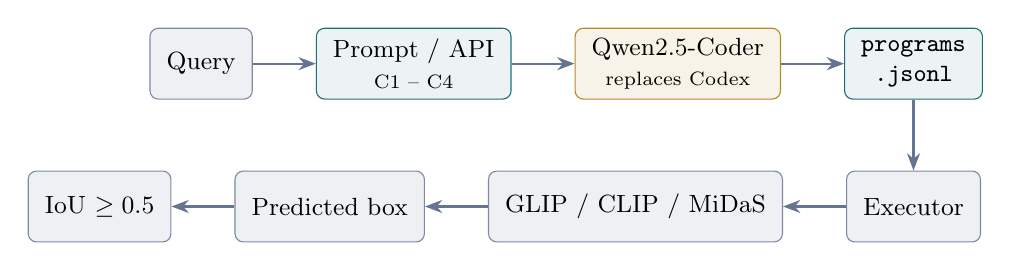
\begin{tikzpicture}[node distance=6mm]
\node[blkg] (q)  {Query};
\node[blkt, right=8mm of q]  (p)  {Prompt / API\\\scriptsize C1 -- C4};
\node[blka, right=8mm of p]  (g)  {Qwen2.5-Coder\\\scriptsize replaces Codex};
\node[blkt, right=8mm of g]  (j)  {\texttt{programs}\\\texttt{.jsonl}};
\node[blkg, below=9mm of j]  (e)  {Executor};
\node[blkg, left=8mm of e]   (m)  {GLIP / CLIP / MiDaS};
\node[blkg, left=8mm of m]   (b)  {Predicted box};
\node[blkg, left=8mm of b]   (i)  {IoU $\geq 0.5$};
\draw[ar] (q)--(p); \draw[ar] (p)--(g); \draw[ar] (g)--(j); \draw[ar] (j)--(e);
\draw[ar] (e)--(m); \draw[ar] (m)--(b); \draw[ar] (b)--(i);
\end{tikzpicture}
\end{center}

\begin{callout}
\emph{``I am not changing the fundamental ViperGPT method. I keep the
query--program--execute pipeline. My experiment studies whether the prompt/API
specification is sufficient for grounding and depth reasoning. I therefore introduce
four controlled conditions, C1 to C4, where each condition adds one specific
intervention.''}
\end{callout}

% =====================================================================
\section{What is passed to the model?}

The generator is asked to write a Python program over an \texttt{ImagePatch}-style
visual API. It never sees the image --- only the query and the API specification.

\begin{center}
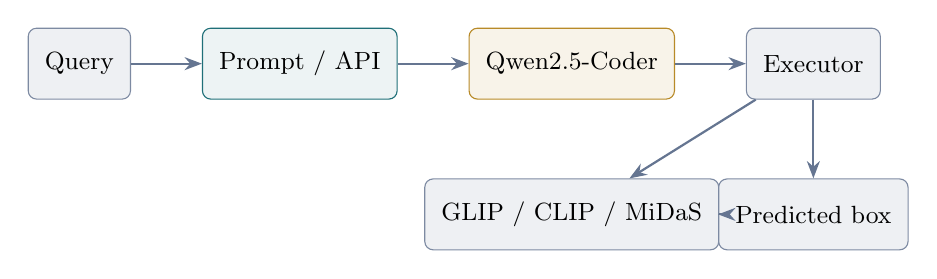
\begin{tikzpicture}[node distance=7mm]
\node[blkg] (q) {Query};
\node[blkt, right=9mm of q] (a) {Prompt / API};
\node[blka, right=9mm of a] (g) {Qwen2.5-Coder};
\node[blkg, right=9mm of g] (x) {Executor};
\node[blkg, below=10mm of g] (v) {GLIP / CLIP / MiDaS};
\node[blkg, below=10mm of x] (o) {Predicted box};
\draw[ar] (q)--(a); \draw[ar] (a)--(g); \draw[ar] (g)--(x);
\draw[ar] (x)--(o); \draw[ar] (x)--(v); \draw[ar] (v)--(o);
\end{tikzpicture}
\end{center}

The important research object is therefore not only the model. It is the
\textbf{interface} between the language model and the visual API.

% =====================================================================
\section{C1 --- released prompt / baseline}

\subsection{What is C1?}

C1 is the released task-agnostic prompt. It provides visual APIs and general Python
instructions, but it does not explicitly say that a grounding program must return an
\texttt{ImagePatch}.

A reported C1 generation for the query \emph{``man on right''} is essentially:

\begin{lstlisting}
def execute_command(image) -> str:
    image_patch = ImagePatch(image)
    man_patches = image_patch.find("man")
    if man_patches:
        man_patch = max(man_patches, key=lambda m: m.right)
        return man_patch.simple_query("Who is on the right?")
    return "No man found."
\end{lstlisting}

The program can be linguistically reasonable, yet it returns a string rather than a
predicted region.

\subsection{Why does this fail for grounding?}

Grounding is evaluated by comparing a predicted box with a ground-truth box using IoU.
A sentence has no predicted box, so its IoU is undefined:
\[
    \text{Correct English answer} \;\not\Rightarrow\; \text{valid grounding output.}
\]

In the reported RefCOCO baseline, \textbf{336 of 500} programs executed to completion
and returned a string, while \textbf{0 of 500} returned a patch. The task-invalid
return rate was $98.8\%$ on RefCOCO and $98.2\%$ on RefCOCO+.

\begin{finding}
\textbf{Interpretation.} C1's $0\%$ is not a crash. The evidence points to an
output-contract failure: the program often produces text instead of an
\texttt{ImagePatch}, so localisation is never reached.
\end{finding}

\begin{callout}
\textbf{Supporting evidence from the specification itself.} The released prompt
contains seven worked examples. Five declare a \texttt{str} return type, one declares
\texttt{List[ImagePatch]}, and exactly one declares \texttt{ImagePatch} --- and that
one is buried inside the docstring of \texttt{compute\_depth}, where a reader seeking
the output contract has no reason to look. No sentence anywhere states that
\texttt{execute\_command} must return an \texttt{ImagePatch}.
\end{callout}

% =====================================================================
\section{C2 --- add the grounding contract}

\begin{center}
\fbox{\parbox{0.86\textwidth}{\centering
\textbf{C2 \;=\; C1 \;+\; explicit grounding contract}}}
\end{center}

C2 adds a small prompt intervention: the function must return the single
\texttt{ImagePatch} referred to by the query; it must not return a string, boolean or
list; and spatial relations must not be dropped. Two worked grounding examples are
also added. Nothing else in this comparison is changed.

For \emph{``man on right''}, the desired pattern becomes:

\begin{lstlisting}
def execute_command(image) -> ImagePatch:
    image_patch = ImagePatch(image)
    man_patches = image_patch.find("man")
    man_patches.sort(key=lambda p: p.horizontal_center)
    return man_patches[-1]
\end{lstlisting}

Now the chain is complete:
\[
    \texttt{ImagePatch} \;\rightarrow\; \text{predicted box} \;\rightarrow\; \text{IoU}.
\]

\subsection{C2 results}

\begin{center}
\begin{tabular}{@{}lrr@{}}
\toprule
\textbf{Metric} & \textbf{C1} & \textbf{C2} \\
\midrule
RefCOCO task-invalid return  & 98.8\% & \up{0.2\%} \\
RefCOCO+ task-invalid return & 98.2\% & \up{0.0\%} \\
RefCOCO accuracy, IoU $\geq 0.5$  & 0.00\% & \up{39.20\%} \\
RefCOCO+ accuracy, IoU $\geq 0.5$ & 0.00\% & \up{31.80\%} \\
RefCOCO patch returns  & 0/500 & 443/500 \\
RefCOCO string returns & 336/500 & 1/500 \\
\bottomrule
\end{tabular}
\end{center}

\begin{finding}
\textbf{Finding.} C2 shows that a large part of the baseline failure is caused by an
underspecified grounding return contract. The model did not suddenly become a better
detector; the interface now clearly states what object type must be returned.
\end{finding}

\begin{callout}
\textbf{Two further pieces of evidence that this is the specification, not the model.}

\smallskip
\emph{Scale.} The same failure occurs at 1.5B, 7B and 32B parameters --- $95.8\%$,
$98.8\%$ and $87.6\%$ task-invalid respectively --- and the same three sentences repair
it at every size. Scaling the generator twentyfold buys about six accuracy points;
stating the contract buys thirty-three to forty-one.

\smallskip
\emph{Format.} Under C1 the model frequently did not define \texttt{execute\_command}
at all, emitting prose instead: $140/500$ on RefCOCO and $212/500$ on RefCOCO+,
against zero under every later condition. The contract disciplines output format as
well as return type.
\end{callout}

% =====================================================================
\section{C3 --- add explicit depth capability}

After C2 the output interface is fixed, but depth and 3D relational queries remain
difficult --- \emph{closest}, \emph{farthest}, \emph{behind}, \emph{in front of},
\emph{between in depth}.

\begin{center}
\fbox{\parbox{0.86\textwidth}{\centering
\textbf{C3 \;=\; C2 \;+\; explicit depth primitives}}}
\end{center}

C3 adds explicit operations:

\begin{center}
\begin{tabular}{@{}ll@{}}
\toprule
\textbf{Primitive} & \textbf{Purpose} \\
\midrule
\texttt{depth\_order()}   & order patches by relative depth \\
\texttt{is\_behind()}     & test a behind relation \\
\texttt{is\_in\_front\_of()} & test a front relation \\
\texttt{is\_between\_3d()} & test a 3D between relation \\
\texttt{distance\_3d()}   & compare relative 3D separation \\
\bottomrule
\end{tabular}
\end{center}

The semantic split introduced by C3 is:
\begin{center}
\begin{tabular}{@{}rcl@{}}
\emph{left / right / above / below} & $\rightarrow$ & 2D image coordinates \\
\emph{closest / farthest / behind / in front} & $\rightarrow$ & depth primitives \\
\end{tabular}
\end{center}

The original API already had \texttt{compute\_depth()}, but it exposed only a scalar.
The reproduction observed \textbf{29} \texttt{compute\_depth} calls against
\textbf{547} \texttt{find} calls. C3 therefore gives the generator a direct vocabulary
for depth relations.

\begin{callout}
\textbf{Why a scalar is not enough.} From one number per object, \emph{``A is behind
B''} is expressible. \emph{``The third-closest person''} requires a total order over a
set; \emph{``between A and B in depth''} requires an interval test over three patches.
Neither is available from a per-patch scalar without the program implementing the
ordering itself --- which the released prompt discourages, since it directs spatial
relations to base Python on image coordinates.
\end{callout}

\subsection{C3 result and problem}

On the RefCOCO+ depth/spatial subset:
\[
    4.26\% \;\longrightarrow\; \up{19.15\%}
\]

However, non-spatial accuracy falls:
\[
    45.97\% \longrightarrow \down{36.02\%} \;\text{(RefCOCO)},
    \qquad
    33.55\% \longrightarrow \down{28.92\%} \;\text{(RefCOCO+)}.
\]

The API-adoption study found \textbf{119} \texttt{depth\_order} calls under C3, where
C1 and C2 had \textbf{zero}. This supports the interpretation that the generator was
reaching for the new capability indiscriminately.

\begin{finding}
\textbf{C3 lesson.} ``Giving the model a capability'' and ``telling the model when
that capability is appropriate'' are different problems. C3 solves the first and
exposes the second.
\end{finding}

% =====================================================================
\section{C4 --- depth capability plus routing rule}

\begin{center}
\fbox{\parbox{0.86\textwidth}{\centering
\textbf{C4 \;=\; C3 \;+\; conditional routing specification}}}
\end{center}

C4 keeps the same depth primitives. The new part is a prompt rule stating that depth
functions should be used \emph{only} when the query actually expresses a depth
relation --- \emph{closest}, \emph{nearest}, \emph{farthest}, \emph{behind},
\emph{in front of}, \emph{between in depth}. The prompt also provides examples of
queries that should \emph{not} use depth. C4 therefore teaches both:

\begin{center}
\textbf{WHEN to use depth} \quad + \quad \textbf{WHEN NOT to use depth}
\end{center}

\begin{center}
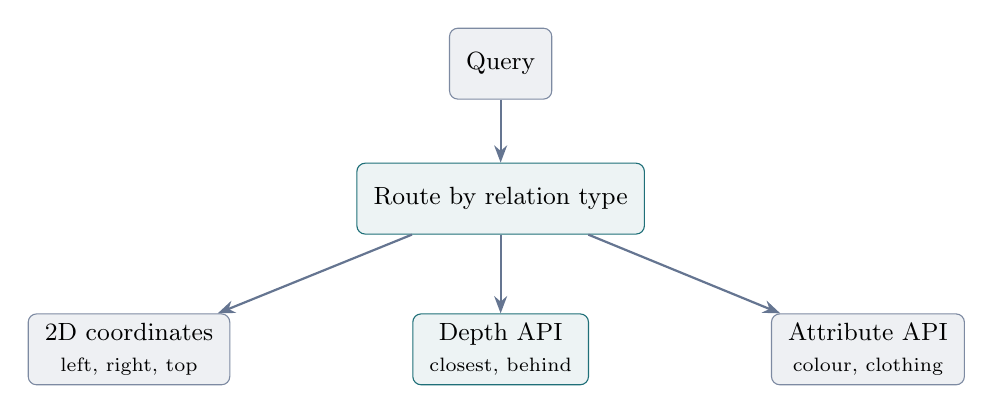
\begin{tikzpicture}[node distance=8mm]
\node[blkg] (q) {Query};
\node[blkt, below=8mm of q] (r) {Route by relation type};
\node[blkg, below left=10mm and 16mm of r] (twod) {2D coordinates\\\scriptsize left, right, top};
\node[blkt, below=10mm of r] (dep) {Depth API\\\scriptsize closest, behind};
\node[blkg, below right=10mm and 16mm of r] (att) {Attribute API\\\scriptsize colour, clothing};
\draw[ar] (q)--(r);
\draw[ar] (r)--(twod); \draw[ar] (r)--(dep); \draw[ar] (r)--(att);
\end{tikzpicture}
\end{center}

\subsection{C4 results}

\begin{center}
\begin{tabular}{@{}lrrrr@{}}
\toprule
\textbf{Dataset / subset} & \textbf{C1} & \textbf{C2} & \textbf{C3} & \textbf{C4} \\
\midrule
RefCOCO+ overall              & 0.00 & 30.80 & 28.00 & \up{37.60} \\
RefCOCO+ spatial, $n = 47$    & 0.00 & 4.26  & 19.15 & \up{21.28} \\
RefCOCO+ non-spatial          & 0.00 & 33.55 & \down{28.92} & \up{39.29} \\
\midrule
RefCOCO overall               & 0.00 & 39.20 & 36.40 & \up{42.00} \\
RefCOCO spatial, $n = 289$    & 0.00 & 34.26 & 36.68 & \up{37.02} \\
RefCOCO non-spatial, $n = 211$& 0.00 & 45.97 & \down{36.02} & \up{48.82} \\
\bottomrule
\end{tabular}
\end{center}

These are accuracy at IoU $\geq 0.5$ for the Qwen2.5-Coder-7B greedy experiment, with
$n = 500$ per cell.

\begin{finding}
\textbf{Main C4 finding.} C4 retains the depth gain while recovering the non-spatial
control performance. RefCOCO overall rises from $39.20\%$ in C2 to $42.00\%$ in C4;
the RefCOCO+ depth/spatial subset rises from $4.26\%$ to $21.28\%$. \textbf{C4 improves
every cell of both datasets relative to C2} --- it is a strict improvement rather than
a trade.
\end{finding}

\subsection{Robustness of the C4 result}

Greedy decoding is deterministic, so variance was estimated separately by sampling at
$T = 0.7$ with three seeds on RefCOCO:

\begin{center}
\begin{tabular}{@{}lccc@{}}
\toprule
\textbf{Condition} & \textbf{overall} & \textbf{spatial} & \textbf{non-spatial} \\
\midrule
C2 contract   & $36.07 \pm 1.75$ & $32.87 \pm 3.35$ & $40.44 \pm 0.72$ \\
C3 + depth    & $34.40 \pm 0.40$ & $34.02 \pm 0.80$ & $34.92 \pm 0.55$ \\
C4 + routing  & $\mathbf{42.07 \pm 0.61}$ & $38.29 \pm 0.72$ & $47.23 \pm 1.19$ \\
\bottomrule
\end{tabular}
\end{center}

Two points follow. First, C4 separates from C2 by $6.0$ points against standard
deviations below two, so the result is not a decoding artefact; note also that C2's
greedy figure ($39.20$) sits $1.8$ standard deviations \emph{above} its own sampled
mean, so the greedy table understates the difference.

Second, and unanticipated: \textbf{the primitives buy stability as well as accuracy}.
Spatial-query standard deviation falls from $\pm 3.35$ under C2 to $\pm 0.72$ under
C4, a factor of $4.6$. Under C2 the generator improvises spatial logic afresh on every
sample --- sometimes sorting by coordinate, sometimes dropping the relation entirely
--- and which it does depends on the seed. Once \texttt{depth\_order} exists there is
one way to express the relation, and the variance collapses.

% =====================================================================
\section{The complete C1--C4 table}

\begin{center}
\begin{tabular}{@{}lcccc@{}}
\toprule
& \textbf{C1} & \textbf{C2} & \textbf{C3} & \textbf{C4} \\
\midrule
Released base prompt                    & Yes      & Yes      & Yes  & Yes \\
Grounding return contract               & No       & Yes      & Yes  & Yes \\
Must return one \texttt{ImagePatch}     & No       & Yes      & Yes  & Yes \\
Spatial relation preservation           & Implicit & Explicit & Explicit & Explicit \\
Explicit depth primitives               & No       & No       & Yes  & Yes \\
Depth routing rule                      & No       & No       & No   & Yes \\
Negative ``do not use depth'' examples  & No       & No       & No   & Yes \\
\bottomrule
\end{tabular}
\end{center}

\begin{center}
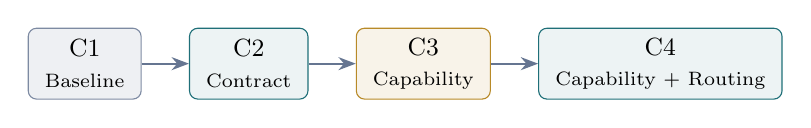
\begin{tikzpicture}[node distance=5mm]
\node[blkg] (c1) {C1\\\scriptsize Baseline};
\node[blkt, right=6mm of c1] (c2) {C2\\\scriptsize Contract};
\node[blka, right=6mm of c2] (c3) {C3\\\scriptsize Capability};
\node[blkt, right=6mm of c3] (c4) {C4\\\scriptsize Capability + Routing};
\draw[ar] (c1)--(c2); \draw[ar] (c2)--(c3); \draw[ar] (c3)--(c4);
\end{tikzpicture}
\end{center}

% =====================================================================
\section{Spatial versus non-spatial --- how to explain it}

The study separates queries into subsets using a relational-term lexicon. Spatial
language includes image-plane relations such as \emph{left}, \emph{right},
\emph{above} and \emph{below}, and depth-related relations such as \emph{closest},
\emph{farthest}, \emph{behind} and \emph{in front}. The depth subset is the smaller
set requiring depth ordering or 3D relational reasoning.

Non-spatial queries act as \textbf{controls}. They matter because if a new depth
capability improves only the target subset while harming other queries, the change is
a trade-off rather than an overall improvement --- which is exactly what C3 turned out
to be.

\begin{callout}
\textbf{Why the two datasets differ.} RefCOCO permits location words; RefCOCO+ forbids
them. A manual audit of all 47 RefCOCO+ spatial queries showed that forbidding location
words removed viewer-frame \emph{directional} expressions but left \emph{depth} ones.
So RefCOCO's spatial subset is predominantly 2D (\emph{``man on right''}) and
RefCOCO+'s is predominantly depth-based (\emph{``man closest to us''}). That is why
they score $34.26$ and $4.26$ respectively under C2, and why the depth primitives help
one far more than the other.
\end{callout}

\begin{callout}
\textbf{The strongest single piece of evidence.} Across three generator sizes ---
1.5B, 7B and 32B --- non-spatial accuracy rises $33.65 \rightarrow 45.97 \rightarrow
48.82$, while spatial accuracy stays flat at $34.95 / 34.26 / 34.95$, on identical
images with identical perception modules. A larger generator writes better programs for
everything \emph{except} spatial relations. If the spatial deficit were a
program-synthesis problem, capacity would help; it demonstrably helps elsewhere. The
bottleneck is therefore the interface, and that is what motivates C3 and C4.
\end{callout}

% =====================================================================
\section{Why the C1--C4 design is a controlled experiment}

Each condition answers a separate question:

\begin{center}
\begin{tabular}{@{}lp{0.72\textwidth}@{}}
\toprule
\textbf{C1} & What happens with the released prompt? \\
\textbf{C2} & Does an explicit grounding output contract fix the grounding failure? \\
\textbf{C3} & Does explicit depth capability improve depth reasoning? \\
\textbf{C4} & Does routing the capability prevent overuse and improve the whole system? \\
\bottomrule
\end{tabular}
\end{center}

This is stronger than changing the entire prompt at once, because it isolates the
effect of each intervention. Each condition is a strict superset of the previous one;
the model, the vision modules, the data and the decoding are held fixed throughout, and
the execution stage re-runs \emph{stored} programs, so a difference in accuracy can
only come from generation.

% =====================================================================
\section{What changed from the original ViperGPT paper?}

\begin{center}
\begin{tabular}{@{}p{0.20\textwidth}p{0.33\textwidth}p{0.39\textwidth}@{}}
\toprule
\textbf{Component} & \textbf{Original / reported setup} & \textbf{This reproduction} \\
\midrule
Generator      & Codex \texttt{code-davinci-002} & Qwen2.5-Coder \\
Prompt study   & Single released specification & C1--C4 controlled conditions \\
Pipeline       & Query $\rightarrow$ program $\rightarrow$ execute &
                 Same core method; generation and execution split by JSONL \\
Depth API      & \texttt{compute\_depth()} scalar &
                 Explicit depth-ordering primitives in C3 / C4 \\
Depth backend  & MiDaS output & Sign corrected and validated \\
Verification   & X-VLM & CLIP ViT-L substitution \\
Environment    & Older published environment & Modernised for H100 execution \\
Threshold      & Paper setup & Re-swept and validated at $0.2$ for detection \\
Scoring        & Paper reporting &
                 Accuracy at IoU $\geq 0.5$ plus mean IoU; missing predictions score 0 \\
\bottomrule
\end{tabular}
\end{center}

\begin{caution}
\textbf{Important claim boundary.} Do \emph{not} call $42.00\%$ a faithful numerical
reproduction of the original Codex result. Codex is retired and several implementation
substitutions are documented. The defensible claim is that the ViperGPT \emph{method}
and the prompt-specification questions are reproduced under a documented modern
implementation.
\end{caution}

\begin{callout}
\textbf{On the metric.} The paper's Table~1 is captioned ``we report accuracy'' while
its column header reads ``IoU (\%)'', and the released evaluator computes mean IoU.
This study reports accuracy at IoU $\geq 0.5$ as primary and mean IoU alongside; on
these runs the two agree to about a point ($42.00$ against $41.81$ for C4 on RefCOCO).
Separately, the released evaluator substitutes the dataset mean box (worth $\approx
22.6$ IoU) for a missing prediction, whereas this study scores an invalid return as
zero. Under the paper's own evaluator, C1 would read $\approx 22.6$ rather than $0.00$
--- the programs are equally invalid either way; what differs is whether the evaluator
conceals the failure.
\end{callout}

% =====================================================================
\section{What is the actual research contribution?}

\begin{enumerate}[leftmargin=1.8em, itemsep=5pt]
\item \textbf{Grounding specification gap.} The released prompt does not explicitly
enforce the required \texttt{ImagePatch} return type. Adding the contract changes
RefCOCO accuracy from $0.00\%$ to $39.20\%$, and the effect is scale-independent
across 1.5B, 7B and 32B generators.

\item \textbf{Depth reasoning gap.} After the grounding contract is fixed,
depth-related queries remain weak. Explicit depth primitives raise the RefCOCO+
depth/spatial subset from $4.26\%$ to $19.15\%$ under C3 and to $21.28\%$ under C4.

\item \textbf{Capability routing.} C3 demonstrates overuse of a new capability; C4 adds
a routing rule and improves \emph{every} reported RefCOCO and RefCOCO+ subset relative
to C2, reaching $42.00\%$ overall and reducing spatial-query variance by $4.6\times$.

\item \textbf{Methodological discipline.} Two results large enough to be attractive
were rejected after control experiments. Capping the detector's candidate set to three
raises RefCOCO accuracy from $42.80\%$ to $57.60\%$ --- but applying the same cap to
C2, which contains \emph{no} depth primitives, yields almost the same gain
($+22.5$ against $+23.9$ points on the spatial subset). The improvement therefore
belongs to the candidate set, not to the method, and is not reported as a result.
\end{enumerate}

% =====================================================================
\section{Summary}

\begin{callout}
\emph{``My experiment has four controlled prompt conditions. C1 is the released
ViperGPT prompt and acts as the baseline. It does not explicitly specify that a
grounding program must return an \texttt{ImagePatch}, so many generated programs
return strings and grounding accuracy is $0\%$.}

\smallskip
\emph{In C2 I add only a grounding contract: the function must return exactly one
\texttt{ImagePatch} and must preserve spatial relations. With the same model and data,
RefCOCO rises from $0\%$ to $39.2\%$.}

\smallskip
\emph{In C3 I address depth reasoning by adding explicit primitives such as
\texttt{depth\_order}, \texttt{is\_behind} and \texttt{is\_in\_front\_of}. Depth-query
performance improves strongly, but non-spatial accuracy falls because the generator
overuses the new capability.}

\smallskip
\emph{Therefore C4 keeps the same depth primitives but adds a routing rule. The prompt
says to use depth functions only for actual depth relations, and gives examples where
depth should not be used. C4 reaches $42.0\%$ overall on RefCOCO and $21.28\%$ on the
RefCOCO+ depth/spatial subset while recovering the non-spatial controls.}

\smallskip
\emph{So the progression is: C1 identifies the specification gap, C2 fixes the output
contract, C3 adds the missing capability, and C4 controls when that capability is
used.''}
\end{callout}

% =====================================================================
\section{Questions and answers}

\begin{description}[leftmargin=0pt, style=unboxed, itemsep=7pt]

\item[\textbf{Why C1--C4?}]
To isolate the effect of each intervention. Changing everything at once would not show
which change caused the improvement.

\item[\textbf{Difference C1 versus C2?}]
C1 leaves the grounding output type implicit; C2 explicitly requires one
\texttt{ImagePatch} and preservation of spatial relations.

\item[\textbf{Difference C2 versus C3?}]
C2 fixes the output interface; C3 adds explicit depth reasoning capability.

\item[\textbf{Difference C3 versus C4?}]
C3 provides depth tools; C4 provides the same tools plus a rule for when they should
and should not be used.

\item[\textbf{Why does C3 hurt non-spatial accuracy?}]
The generator overuses the newly exposed depth capability on queries that should use
2D coordinates or attribute verification. \texttt{depth\_order} was called 119 times on
RefCOCO, where most queries need no depth at all.

\item[\textbf{Why is C4 better?}]
It preserves the depth capability while constraining its use, so the target subset
improves without the collateral loss --- and every other subset improves as well.

\item[\textbf{Is the Qwen replacement your contribution?}]
No. It is a necessary present-day reproduction substitution because Codex is retired.
The research contribution is the controlled diagnosis of specification gaps and
capability routing.

\item[\textbf{Did C1 really fail?}]
It failed as a grounding interface. Many programs executed successfully and returned
strings, but a string has no predicted box and therefore cannot receive an IoU score.
This is why the failure is described as a specification failure rather than a crash.

\item[\textbf{Is the improvement just the smaller candidate set?}]
No, and this was tested directly. Capping the detector's candidates does raise accuracy
substantially, but a control condition without any depth primitives gains almost as
much, so that gain is attributable to the candidate set rather than to the method. It
is therefore disabled in all reported results.

\item[\textbf{How do you know the depth signal is correct?}]
It was validated against ground-truth boxes with the detector removed entirely. With
the corrected sign the annotated target lands at the correct depth extreme in $20$ of
$25$ cases; without it, in $2$ of $25$, against a chance level of $26\%$. A score
\emph{below} chance indicates an inverted signal rather than a weak one.

\item[\textbf{What is your strongest conclusion?}]
Capability and specification are separate concerns. A model needs both the capability
and a clear rule for when that capability applies.

\end{description}

% =====================================================================
\section{Final}

\begin{center}
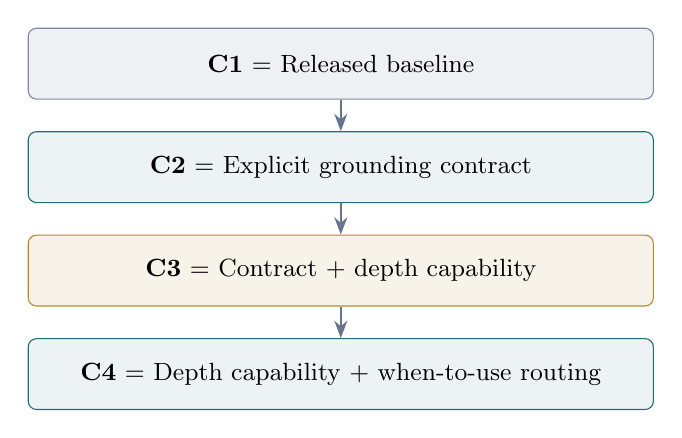
\begin{tikzpicture}[node distance=4mm]
\node[blkg, text width=0.62\textwidth] (a) {\textbf{C1} = Released baseline};
\node[blkt, below=4mm of a, text width=0.62\textwidth] (b) {\textbf{C2} = Explicit grounding contract};
\node[blka, below=4mm of b, text width=0.62\textwidth] (c) {\textbf{C3} = Contract + depth capability};
\node[blkt, below=4mm of c, text width=0.62\textwidth] (d) {\textbf{C4} = Depth capability + when-to-use routing};
\draw[ar] (a)--(b); \draw[ar] (b)--(c); \draw[ar] (c)--(d);
\end{tikzpicture}
\end{center}

\begin{center}\small
C1 identifies the problem $\rightarrow$ C2 fixes the contract $\rightarrow$
C3 adds capability $\rightarrow$ C4 controls when it is used.
\end{center}

\begin{finding}
\textbf{Final.} The key result is not merely that C4 has a higher number. The
controlled progression shows \emph{why}: C2 fixes an output-interface omission, C3 adds
a missing depth capability, and C4 demonstrates that the capability must be accompanied
by an explicit condition describing when it applies.
\end{finding}

\vspace{10pt}
\hrule
\vspace{4pt}
{\footnotesize\color{midgrey}
All figures reported here are traceable to stored run summaries and scheduler job
identifiers. The C2 return-count figures (336 string returns, 443 patch returns) and
the RefCOCO+ C2 accuracy of $31.80\%$ come from the Milestone~2 execution set; the
C1--C4 comparison table in Section~7 comes from the Milestone~3 set, in which the
corresponding values are 332, 444 and $30.80\%$. The two sets differ only in run
provenance and not in any conclusion drawn.}

\end{document}
